\subsection{Case Study: Synthetic Data vs. Real Sensor Noise \quad / \quad \textthai{กรณีศึกษา: ข้อมูลจำลองและสัญญาณรบกวนของเซนเซอร์}}
In this chapter's practical section, we will use Python to simulate an ideal oscillator (Synthetic Data) and then inject realistic Gaussian noise to mimic experimental sensor data (Real-world Modeling). This hybrid approach is common in physics-informed machine learning, where we use synthetic theory to "pre-train" models before applying them to noisy experimental datasets from sources like LIGO.

\begin{pythonbox}{Synthetic Oscillator with Gaussian Noise (scripts/ch1/harmonic\_oscillator.py)}
\begin{lstlisting}
import numpy as np
import matplotlib.pyplot as plt

# 1. Theoretical Grid (Synthetic)
t = np.linspace(0, 10, 500)
x_true = np.cos(2 * np.pi * 0.5 * t) # Frequency = 0.5 Hz

# 2. Experimental Reality (Noise Injection)
# Mimicking sensor inaccuracies at 5% noise level
noise = 0.05 * np.random.normal(size=t.shape)
x_observed = x_true + noise

# 3. Visualization
plt.plot(t, x_true, label='Theoretical (Clean)')
plt.scatter(t, x_observed, color='red', alpha=0.3, s=10, label='Sensor Observation (Noisy)')
plt.legend()
plt.show()
\end{lstlisting}
\end{pythonbox}

\subsubsection*{Code Anatomy \quad / \quad \textthai{การวิเคราะห์โค้ด}}
\begin{paracol}{2}
\textbf{Synthetic Generation}: The \texttt{x\_true} calculation represents our "perfect" physical model. It follows the derivation in Section 1.2 exactly. In AI training, this serves as our "Ground Truth."\index{Ground Truth@ข้อมูลจริง (Ground Truth)}

\switchcolumn

\begin{thai}
\textbf{การสร้างข้อมูลจำลอง}: การคำนวณ \texttt{x\_true} แสดงถึงแบบจำลองทางกายภาพที่ "สมบูรณ์แบบ" ของเรา โดยเป็นไปตามการอนุมานในส่วนที่ 1.2 อย่างแม่นยำ ในการฝึก AI สิ่งนี้ทำหน้าที่เป็น "ข้อมูลจริง (Ground Truth)"
\end{thai}
\end{paracol}

\begin{paracol}{2}
\textbf{Noise Injection}\index{Noise Injection@การใส่สัญญาณรบกวน (Noise Injection)}: Real physical sensors are never perfect. By adding \texttt{np.random.normal}, we simulate the thermal noise found in electronics. Learning to filter this noise is the primary goal of \textbf{Deep Denoising Autoencoders} used in astrophysics today.

\switchcolumn

\begin{thai}
\textbf{การใส่สัญญาณรบกวน (Noise Injection)}: เซนเซอร์ทางกายภาพจริงๆ ไม่สมบูรณ์แบบเสมอไป การเพิ่ม \texttt{np.random.normal} ช่วยให้เราจำลองสัญญาณรบกวนจากความร้อน (Thermal Noise) ที่พบในอุปกรณ์อิเล็กทรอนิกส์ การเรียนรู้เพื่อกรองสัญญาณรบกวนนี้เป็นเป้าหมายหลักของ \textbf{Deep Denoising Autoencoders} ที่ใช้ในวิชาดาราศาสตร์ฟิสิกส์ในปัจจุบัน
\end{thai}
\end{paracol}

\subsubsection*{Results and Analysis \quad / \quad \textthai{ผลลัพธ์และการวิเคราะห์}}
\begin{paracol}{2}
The following figure illustrates the outcome of our harmonic oscillator simulation. The left panel shows the oscillation of position over time, while the right panel displays the phase space—the relationship between position and velocity. In a perfect simulation (no numerical drift), the phase space should be a closed ellipse, representing the conservation of total energy ($E = T + V = \text{const}$).

\switchcolumn

\begin{thai}
รูปด้านล่างแสดงผลลัพธ์จากการจำลองตัวสั่นพ้องแบบฮาร์มอนิกของเรา โดยแผงด้านซ้ายแสดงการแกว่งของตำแหน่งตามเวลา ในขณะที่แผงด้านขวาแสดงระวางเฟส (Phase Space) ซึ่งเป็นความสัมพันธ์ระหว่างตำแหน่งและความเร็ว ในการจำลองที่สมบูรณ์แบบ (ไม่มีความคลาดเคลื่อนทางตัวเลข) ระวางเฟสควรจะเป็นวงรีปิด ซึ่งแสดงถึงการอนุรักษ์พลังงานรวม ($E = T + V = \text{คงที่}$)
\end{thai}
\end{paracol}

\begin{figure}[h]
    \centering
    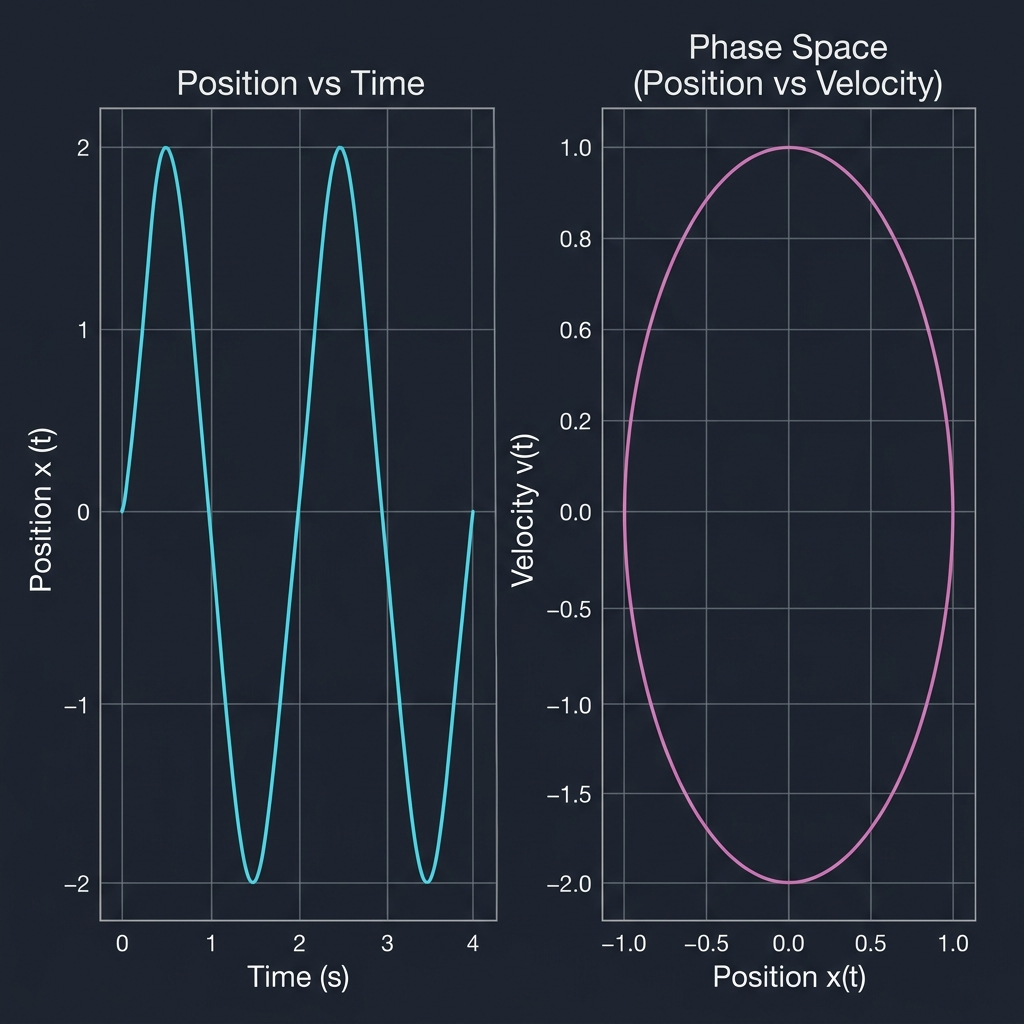
\includegraphics[width=0.9\textwidth]{assets/ch1_oscillator_results.png}
    \caption{Numerical Simulation Results for a Simple Harmonic Oscillator ($k=1, m=1$)}
    \label{fig:oscillator_results}
\end{figure}

\begin{paracol}{2}
To better understand the underlying data, the table below provides a sample of the first 10 time steps of the simulation. Notice how the velocity starts to decrease as the restoring force pulls the mass back toward the equilibrium position ($x=0$).

\switchcolumn

\begin{thai}
เพื่อให้เข้าใจข้อมูลพื้นฐานได้ดียิ่งขึ้น ตารางด้านล่างแสดงตัวอย่างของ 10 ขั้นตอนเวลาแรกของการจำลอง สังเกตว่าความเร็วเริ่มลดลงอย่างไรเมื่อแรงดึงกลับดึงมวลกลับไปที่ตำแหน่งสมดุล ($x=0$)
\end{thai}
\end{paracol}

\begin{table}[h]
    \centering
    \caption{Numerical Simulation Data Sample}
    \begin{tabular}{ccc}
        \toprule
        Time (s) & Position (m) & Velocity (m/s) \\
        \midrule
        0.00 & 1.0000 & 0.0000 \\
        0.10 & 0.9950 & -0.0998 \\
        0.20 & 0.9801 & -0.1987 \\
        0.30 & 0.9553 & -0.2955 \\
        0.40 & 0.9211 & -0.3894 \\
        0.50 & 0.8776 & -0.4794 \\
        0.60 & 0.8253 & -0.5646 \\
        0.70 & 0.7648 & -0.6442 \\
        0.80 & 0.6967 & -0.7174 \\
        0.90 & 0.6216 & -0.7833 \\
        \bottomrule
    \end{tabular}
\end{table}
